\documentclass[a4paper,11pt]{article}

% \usepackage[smartEllipses]{markdown}
% \usepackage[hashEnumerators,smartEllipses]{markdown}
% \usepackage[hashEnumerators,smartEllipses,hybrid]{markdown}
\usepackage[hybrid]{markdown}
\usepackage[export]{adjustbox} % рамки вокруг фото
\usepackage{minted} % Для вставки кода
% \usepackage{xpatch}
% \xpretocmd{\inputminted}{\par\vspace{1em}}{}{}
% \xapptocmd{\inputminted}{\par\vspace{1em}}{}{}
% \usepackage{indentfirst}
% \setlength{\parindent}{0pt} % Отключает отступ в начале каждого абзаца
\usepackage{parskip} % убрать красную строку и добавить вертикальный отступ между абзацами


%%% Мои команды
\newcommand{\insertMyCode}[2]{ % вставка кода
    % #1 — язык
    % #2 — путь до файла
    \inputminted[
    % framesep=2mm,
    baselinestretch=1.2,
    bgcolor=LightGray!30,
    fontsize=\footnotesize,
    linenos
    ]{#1}{#2}
}


%%% Работа с русским языком
\usepackage{cmap} % поиск в PDF
\usepackage{mathtext} % русские буквы в фомулах
\usepackage[T2A]{fontenc} % кодировка
\usepackage[utf8]{inputenc} % кодировка исходного текста
\usepackage[english,russian]{babel} % локализация и переносы

%%% Дополнительная работа с математикой
\usepackage{amsmath,amsfonts,amssymb,amsthm,mathtools} % AMS
\usepackage{icomma} % "Умная" запятая: $0,2$ —- число, $0, 2$ —- перечисление

%%% Перенос знаков в формулах (по Львовскому)
\newcommand*{\hm}[1]{#1\nobreak\discretionary{}
{\hbox{$\mathsurround=0pt #1$}}{}}

%%% Работа с картинками
\usepackage{graphicx} % Для вставки рисунков
\graphicspath{{images/}} % папки с картинками
% \setlength\fboxsep{3pt} % Отступ рамки \fbox{} от рисунка
% \setlength\fboxrule{1pt} % Толщина линий рамки \fbox{}
% \usepackage{wrapfig} % Обтекание рисунков текстом

%%% Работа с таблицами
\usepackage{array,tabularx,tabulary,booktabs} % Дополнительная работа с таблицами
\usepackage{longtable} % Длинные таблицы
\usepackage{multirow} % Слияние строк в таблице

%%% Теоремы
% \theoremstyle{plain} % Это стиль по умолчанию, его можно не переопределять.
\newtheorem{theorem}{Теорема}[section]
\newtheorem{proposition}[theorem]{Утверждение}

\theoremstyle{definition} % "Определение"
\newtheorem{corollary}{Следствие}[theorem]
\newtheorem{problem}{Задача}[section]

\theoremstyle{remark} % "Примечание"
\newtheorem*{nonum}{Решение}

%%% Программирование
\usepackage{etoolbox} % логические операторы

%%% Страница
% \usepackage{extsizes} % Возможность сделать 14-й шрифт % конфликт с parskip
\usepackage{geometry} % Простой способ задавать поля
\geometry{top=25mm}
\geometry{bottom=35mm}
\geometry{left=20mm}
\geometry{right=20mm}

\usepackage{fancyhdr} % Колонтитулы
\pagestyle{fancy}
\renewcommand{\headrulewidth}{0mm} % Толщина линейки, отчеркивающей верхний колонтитул
% \lfoot{Нижний левый}
% \rfoot{Нижний правый}
% \rhead{Верхний правый}
% \chead{Верхний в центре}
% \lhead{Верхний левый}
\cfoot % По умолчанию здесь номер страницы

\usepackage{lastpage} % Узнать, сколько всего страниц в документе.

\usepackage{soul} % Модификаторы начертания

\usepackage{setspace} % Интерлиньяж
%\onehalfspacing % Интерлиньяж 1.5
%\doublespacing % Интерлиньяж 2
%\singlespacing % Интерлиньяж 1

\usepackage{hyperref}
\usepackage[usenames,dvipsnames,svgnames,table,rgb]{xcolor}
\hypersetup{ % Гиперссылки
unicode=true, % русские буквы в раздела PDF
pdftitle={Заголовок}, % Заголовок
pdfauthor={Автор}, % Автор
pdfsubject={Тема}, % Тема
pdfcreator={Создатель}, % Создатель
pdfproducer={Производитель}, % Производитель
pdfkeywords={keyword1} {key2} {key3}, % Ключевые слова
colorlinks=true, % false: ссылки в рамках; true: цветные ссылки
linkcolor=red, % внутренние ссылки
citecolor=green, % на библиографию
filecolor=magenta, % на файлы
urlcolor=cyan % на URL
}

\usepackage{multicol} % Несколько колонок

%%% Хз что это (потом разобраться)
% \usepackage{upgreek}
\usepackage{cite}
\usepackage{csquotes} % Еще инструменты для ссылок
%Смотри источник 1 \cite{qwerty,Fama,Fama2}.
%\renewcommand{\refname}{Список источников}  % По умолчанию %"Список литературы" (article)
%\renewcommand{\bibname}{Литература}  % По умолчанию "Литература" (book и report)
%\renewcommand{\familydefault}{\sfdefault} % Начертание шрифта

\begin{document}


\begin{titlepage} % начало титульной страницы
\pagestyle{empty}
\begin{center}

\Large
\textbf{Федеральное государственное автономное образовательное учреждение высшего образования\\
«Национальный исследовательский университет\\
«Высшая школа экономики»}\\
\vspace{5mm}

\Large
Образовательная программа \\
«Прикладная математика»
\vspace{40mm}

\Large
\textbf{ОТЧЕТ} \\
\textbf{По лабораторной работе № 1} \\
\vspace{5mm}
\Large По предмету \\
\LARGE\textbf{«Численные методы»} \\
\vspace{5mm}
\Large По теме \\
\LARGE\textbf{«Теория погрешностей и машинная арифметика»}
\end{center}

\begin{center}
\vfill

\large
\begin{flushright}
\textbf{Выполнил} \\
студент группы БПМ211 \\
Кудряшов Максим Дмитриевич \\
\end{flushright}

\large
\begin{flushright}
\textbf{Проверил} \\
Брандышев Петр Евгеньевич \\
\end{flushright}

\large
\vspace{20mm}
Москва - 2024
\end{center}
\end{titlepage} % конец титульной страницы

\newpage
\tableofcontents
\newpage

\section{3.1.8}

\subsection{Постановка задачи}

Дана система уравнений $A x=b$ порядка $n = 6$. 
Исследовать зависимость погрешности решения $x$ от погрешностей правой части системы $b$.

$$A_{ij} = \frac{1}{\sqrt{c_{ij}^2 + 0.58 c_{ij}}}$$

$$b_i = N$$

$$c_{ij} = 0.1 N i j$$

$$N = 8$$

\subsection{Теория}

\subsection{аналитическое решение тестового примера и результат вычислительного эксперимента по тесту}

\subsection{Код на Python}
\insertMyCode{python3}{../3.1.8.py}

\subsection{Результаты}

\insertMyCode{text}{../3.1.8.txt}
\begin{figure}[h]
    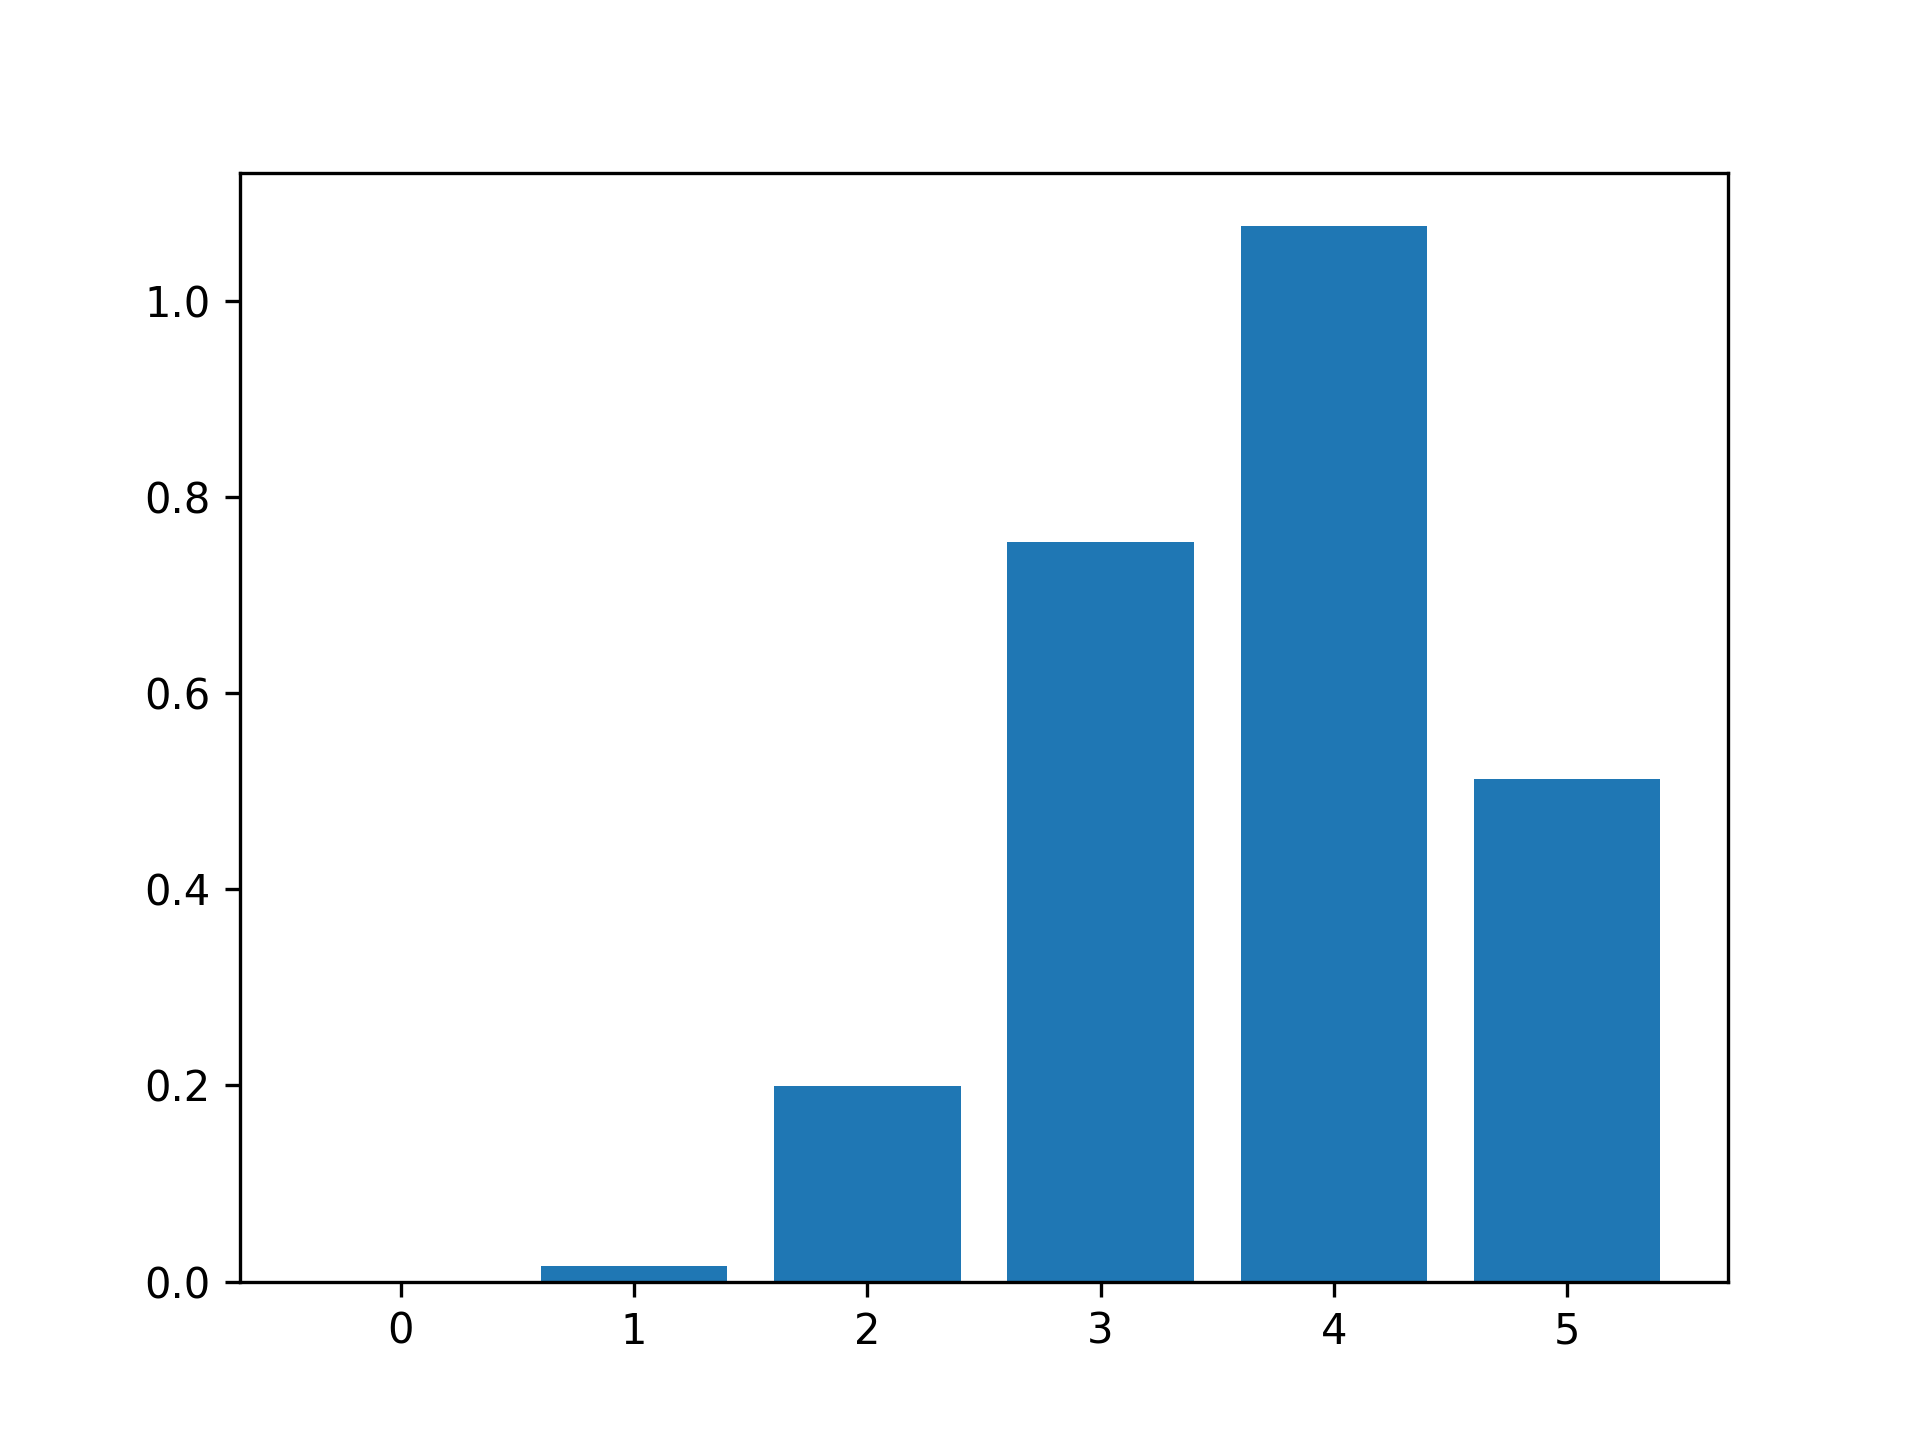
\includegraphics[width=0.5\linewidth]{../../3.1.8.png}
\end{figure}



\section{3.2}

\section{3.8.2}

\end{document}
